\documentclass[aps,prl,onecolumn,superscriptaddress,english,notitlepage]{revtex4-1}

\usepackage[T1]{fontenc}
\usepackage[latin9]{inputenc}
\usepackage{babel}
\usepackage{amsmath}
\usepackage{amssymb}
\usepackage{wasysym}
\usepackage{graphicx}
\usepackage{xcolor}
\usepackage{graphicx}
\usepackage[section]{placeins}

\usepackage[linktocpage=true,
  colorlinks=true, 
  pdfborder={0 0 0},
  linkcolor=blue,
  citecolor=red,
  filecolor=yellow,
  urlcolor=blue,
  bookmarks,
  pdfauthor={},
]{hyperref}

\usepackage{ulem}

\newcommand{\Oxford}{Department of Materials, University of Oxford, Parks Road, Oxford OX1 3PH, 
United Kingdom}
\newcommand{\Kings}{King's College London, Physics Department, Strand, London WC2R 2LS, United Kingdom}
\newcommand{\Binghamton}{Department of Physics, Applied Physics and Astronomy, Binghamton 
University-SUNY, Binghamton, New York 13902, USA}

\renewcommand{\thefigure}{S\arabic{figure}}

\begin{document}

\title{Supplemental Material \vspace{0.2cm}\\ 
Origin of superconductivity and latent charge density wave in NbS$_2$}

\author{Christoph Heil}      \affiliation{\Oxford}
\author{Samuel Ponc\'{e}}    \affiliation{\Oxford}
\author{Henry Lambert}       \altaffiliation[present address: ]{\Kings} \affiliation{\Oxford}
\author{Martin Schlipf}     \affiliation{\Oxford}
\author{Elena R. Margine}    \affiliation{\Binghamton}
\author{Feliciano Giustino}  \email{feliciano.giustino@materials.ox.ax.uk} \affiliation{\Oxford}

\date{\today}

\maketitle

% \null
% \vfill

  \begin{figure}[htbp]
  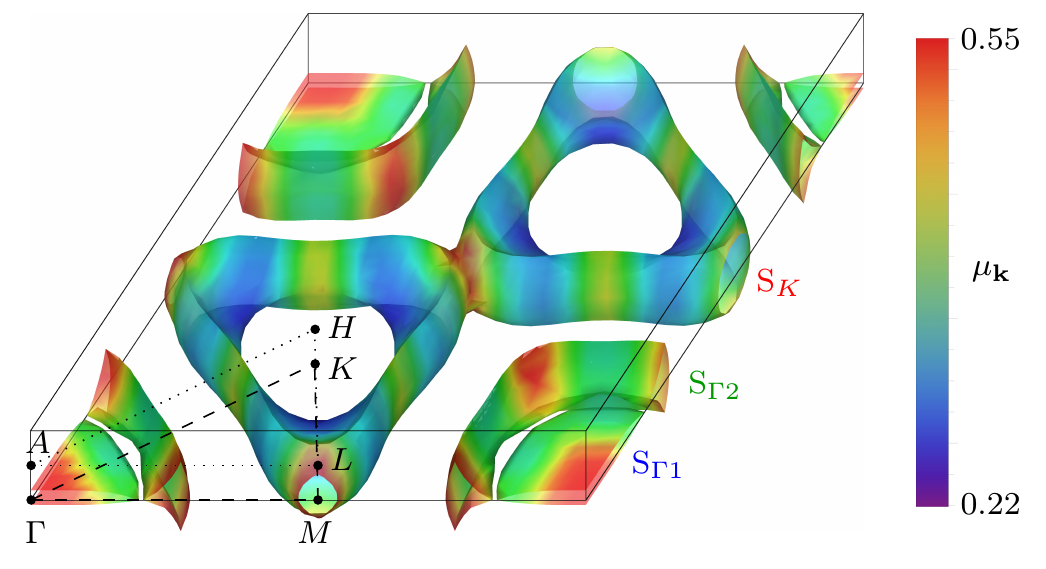
\includegraphics[width=0.5\textwidth]{figS1}
  \caption{(Color online) Distribution of the pair-breaking screened Coulomb interaction $\mu_k$ on the Fermi surface, with blue indicating the lowest value and red the highest. $\mu_\mathbf{k}$ is defined as the Fermi-surface average of the screened Coulomb interaction W: $\mu_\mathbf{k}=N_{\rm F} \langle\,  \langle {\bf k},-{\bf k} |W| {\bf k}',-{\bf k}' \rangle \, \rangle_\text{FS}$.}
  \end{figure}

% \null
% \vfill
% \clearpage  
% \newpage

% \null
% \vfill
\section{Anharmonic phonon calculations}


Here we describe our approach to determine the vibrational properties of 2$H$-NbS$_2$ including anharmonic effects.
First, we perform density-functional perturbation theory (DFPT) calculations in the harmonic approximation to obtain the vibrational eigenmodes $\mathbf{e}_{\mathbf{q}, \kappa}^\nu$ and eigenfrequencies $\omega_{\mathbf{q,\nu}}$ of atom $\kappa$ and mode $\nu$ at wavevector $\mathbf{q}$ on a uniform $N_1^p \times N_2^p \times N_3^p$ grid centered at $\Gamma$. The corresponding dynamical matrix in the Bloch representation is given by:

\begin{equation}
\label{eq1}
 D^\text{ph}_{\mathbf{q},\mu \nu} = \langle \mathbf{q} \mu | \hat{D}^\text{ph} | \mathbf{q} \nu \rangle = \delta_{\mu \nu} \omega^2_{\mathbf{q},\nu}.
\end{equation}

In the phonon Wannier representation the same matrix can be written as \cite{giustino_electron-phonon_2007}:

\begin{equation}
\label{eq2}
 D^\text{ph}_{\mathbf{R}_p,\mathbf{R}'_p} = \langle \mathbf{R}_p | \hat{D}^\text{ph} | \mathbf{R}_p' \rangle = \sum \limits_\mathbf{q} e^{-i \mathbf{q} \cdot (\mathbf{R}'_{p} - \mathbf{R}_{p})} E_\mathbf{q} D^\text{ph}_{\mathbf{q}} E_\mathbf{q}^\dagger.
\end{equation}

Here $\mathbf{R}_p$ denote the lattice vectors and we have rewritten the vibrational eigenvectors as square matrices $(E_\mathbf{q})_{\mu \nu}$. The phonon eigenmodes and eigenfrequencies at an arbitrary wavevector $\mathbf{q}'$ can then be obtained by inverting Eq.~(\ref{eq2}), i.e.:

\begin{equation}
\label{eq3}
 D^\text{ph}_{\mathbf{q}'} = E_{\mathbf{q}'}^\dagger \left(\frac{1}{N_p} \sum \limits_{\mathbf{R}_p} e^{-i \mathbf{q}' \cdot \mathbf{R}_{p}}  D^\text{ph}_{\mathbf{0}_p,\mathbf{R}_p} \right) E_{\mathbf{q}'}~.
\end{equation} 

In order to calculate the eigenfrequencies and eigenmodes for a wavevector $\mathbf{q}'$, one first has to Fourier interpolate the dynamical matrix in Wannier representation [the term in brackets of Eq.~(\ref{eq3})] and then diagonalize the resulting matrix. For further details we refer the reader to Ref.~\onlinecite{giustino_electron-phonon_2007}.

To calculate phonon dispersion relations in the presence of anharmonicity, 
we retain the (harmonic) DFPT eigenmodes $(E_\mathbf{q})_{\mu \nu}$, and we correct the
eigenfrequencies $\omega_{\bf q,\nu}$ in Eq.~(\ref{eq1}) using calculations for anharmonic 
potential energy surfaces. The interatomic force constants in Eq.~(\ref{eq2}) are then
computed using the modified frequencies, and the Fourier interpolation in Eq.~(\ref{eq3})
is finally used to reconstruct the band structures.

The anharmonic corrections to the vibrational frequencies are calculated as follows.
We first compute the vibrational eigenmodes for a supercell constructed so as to fold the 
desired wavevector $\mathbf{q}$ onto the $\Gamma$ point. 
Then we evaluate the adiabatic potential energy surface (APES) by calculating 
the total energy of the system as a function of the atomic displacements according to the selected 
phonon eigenvector, as in the frozen-phonon approach~\cite{lam_ab_1982}. The atomic displacements are 
given by:

\begin{equation}
 \Delta \tau_{\kappa,\alpha}(x) = \sqrt{\frac{M_0}{M_\kappa}} e_{\kappa,\alpha} x,
\end{equation}

where $M_\kappa$ is the nuclear mass of atom $\kappa$ and $M_0$ the proton mass. 
We calculate the eigenvalues of the APES generated by this displacement; this is achieved
by solving a one-dimensional Schr\"{o}dinger equation, following the same procedure outlined in 
Ref.~\onlinecite{giustino_materials_2014}, Sec.~8.2.

As an example, the anharmonic APES for the lowest-energy phonon of NbS$_2$ at $M$ 
is shown as a solid black line in Fig.~S2(a). For comparison we also show the harmonic potential
as a dashed red line.
The square moduli of the calculated wavefunctions, vertically shifted by their eigenvalue for clarity, 
are shown as solid colored lines in Fig.~S2(a). We performed similar calculations for the wavevectors at 
$2/3 \Gamma M$ and $L$.

To check the sensitivity of $T_{\rm c}$ to the frequencies of the anharmonic phonons, 
we have repeated the Migdal-Eliashberg calculations by artificially shifting the frequencies 
of the anharmonic modes, as shown in  Fig.~S7. 
We find that $T_{\rm c}$ is relatively insensitive to small changes in these frequencies.
For example, changing the frequencies of both anharmonic modes by $-4.5$\;meV, so as to set the frequency of the first phonon mode at $M$ almost to zero, reduces $T_{\rm c}$ by only 12\%. We also checked that the results are insensitive to
the ordering of the lowest two vibrational modes.

The approach just described includes by construction phonon-phonon interactions within the
{\it same} harmonic eigenmode, but it neglects phonon-phonon interactions between {\it different}
eigenmodes. In order to check the magnitude of the inter-mode couplings it is necessary to
consider a multi-dimensional APES, whereby the atomic displacements are expanded in terms 
of multiple normal coordinates:

\begin{equation}
 \Delta \tau_{\kappa,\alpha}(x_{\nu_1}, ..., x_{\nu_N}) = \sqrt{\frac{M_0}{M_\kappa}} \left( e^{\nu_1}_{\kappa,\alpha} x_{\nu_1} + ... + e^{\nu_N}_{\kappa,\alpha} x_{\nu_N} \right)~.
\end{equation}

Since this operation is computationally prohibitive, we tested the coupling between the two 
anharmonic phonons at the $M$ point by calculating two-dimensional potential energy surfaces.
The square moduli 
of the first three eigenstates of the 2D-APES are shown in Fig.~S2(c)-(e). The calculated phonon frequencies,
$4.4$\;meV and $8.6$\;meV, are in good agreement with the values that we obtained by using 1D-APES
calculations, namely
$4.7$\;meV and $8.1$\;meV respectively. This favorable comparison indicates that for the purposes
of the present work it is legitimate to consider 1D-APES calculations of anharmonic corrections.

When compared to perturbative calculations of anharmonicity, the approach that we employ here
carries the advantage that anharmonicity (within a single eigenmode) is included to all orders.
Furthermore, when used in conjunction with standard Fourier interpolation techniques of
the interatomic force constants, this method can provide complete phonon dispersion relations. The inclusion
of inter-mode anharmonic coupling is also possible by considering multi-dimensional APES, although
these calculations can become very time-consuming.

The disadvantages of the method used here are: (i) the procedure is limited to 
$\mathbf{q}$-vectors which are commensurate with small supercells (most typically high-symmetry
points in the Brillouin zone); (ii) inter-mode anharmonic phonon-phonon interactions can only 
be considered for a small subset of phonon modes.

In contrast, self-consistent 
approaches to anharmonic 
phonons~\cite{born_fest._1951,hooton_li._1955,koehler_theory_1966,souvatzis_entropy_2008,errea_first-principles_2013} 
automatically incorporate both intra-mode and inter-mode anharmonic couplings.
In addition, these approaches allows for the incorporation of temperature in the calculated
phonon spectra~\cite{souvatzis_entropy_2008}. Therefore self-consistent methods are more
general than the present approach, but come at an increased computational cost.
  
  \begin{figure}[htbp]
  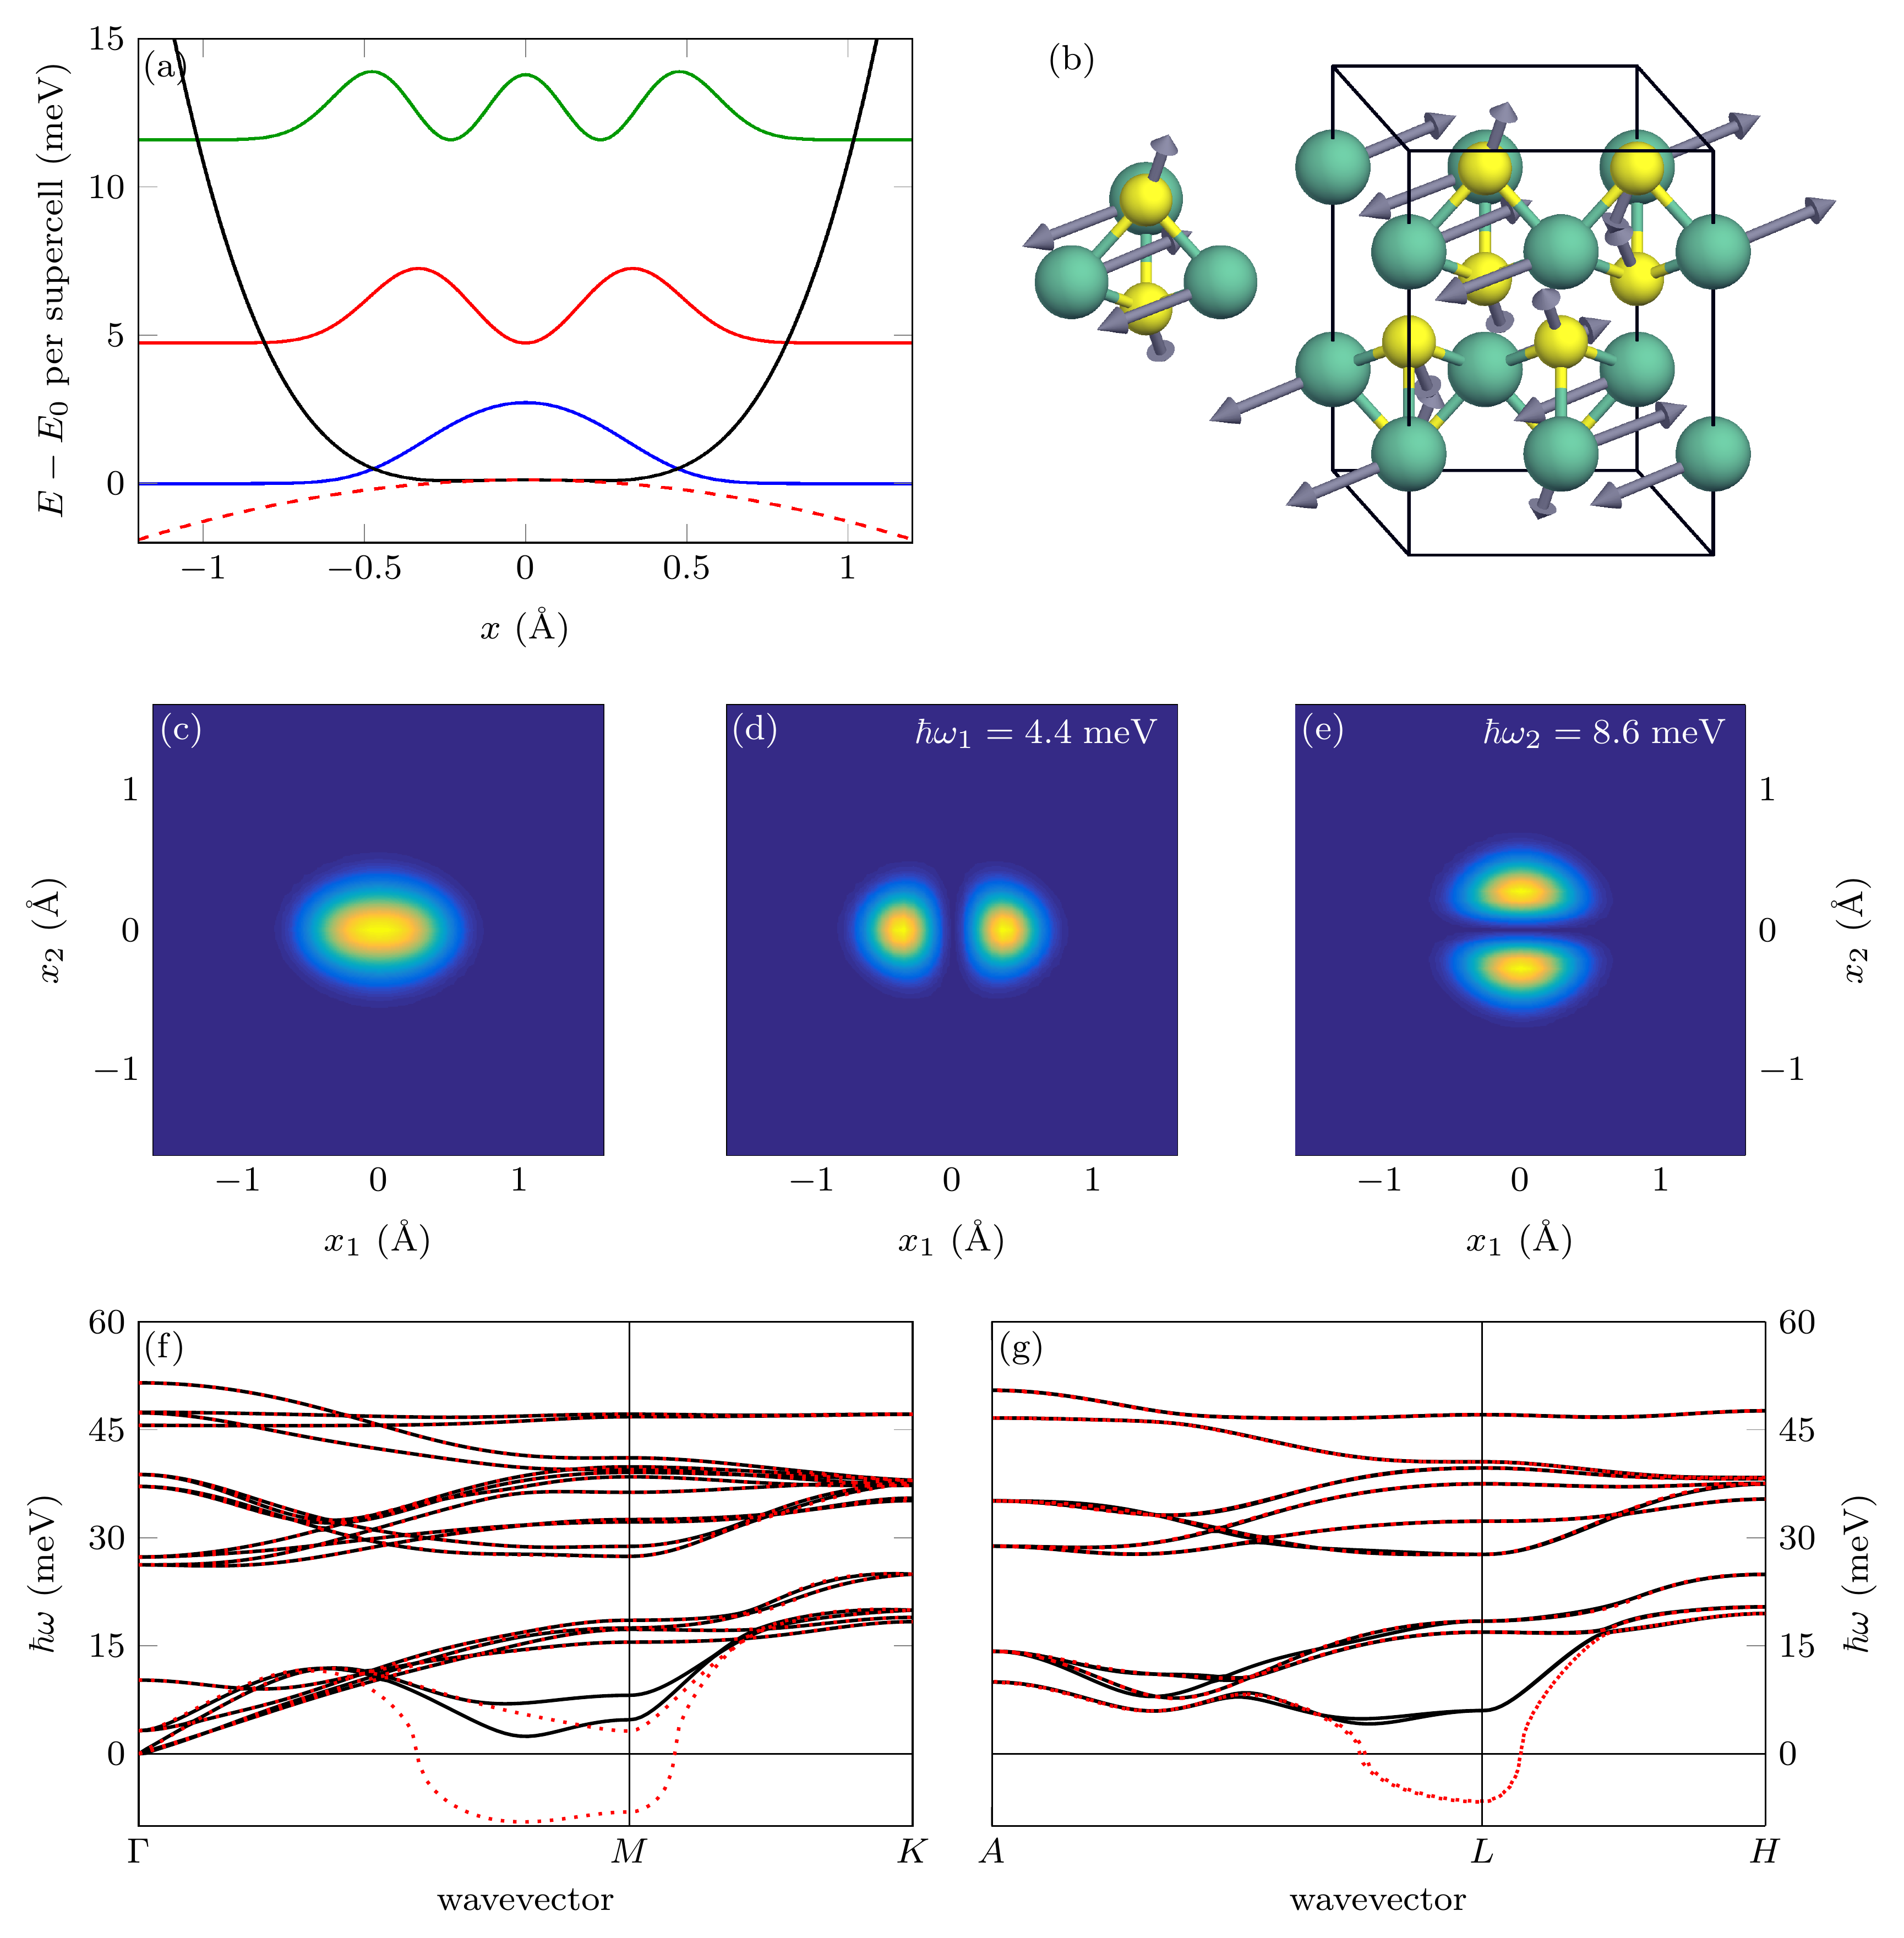
\includegraphics[width=0.8\textwidth]{figS2}
  \caption{(Color online) 
  (a) Adiabatic potential energy surface (APES) of 2$H$-NbS$_2$, calculated along the normal mode coordinate $x$ corresponding to the lowest-energy mode at $M$, fitted up to 8$^\text{th}$ order (solid black line). The dashed red line shows the harmonic part of the APES.
  %
  The square moduli of the wavefunctions corresponding to the APES in panel (a) are shown in order of increasing energy as solid colored lines. These curves have been vertically shifted by their energy eigenvalue. The calculation corresponding to panel (a) was carried out for a $2\times1\times1$ supercell so as to fold $M$ into $\Gamma$, with a uniform $18 \times 36 \times 12$ $\mathbf{k}$-grid and an electronic smearing parameter of $0.005$\;Ry. We performed similar calculations for the phonons at $2/3 \,\Gamma M$ and at $L$, obtaining similar results. 
  %
  (b) Atomic displacement pattern corresponding to the lowest-energy phonon at $M$, showing the vibration of the Nb$_3$S$_2$ trigonal bipyramidal units.
  %
  (c)-(e) Square moduli of the first three wavefunctions calculated for the 2-dimensional APES (again fitted up to 8$^\text{th}$ order in both coordinates), taking into account the coupling between the two anharmonic phonon modes at $M$. The calculated eigenfrequencies are in good agreement with the uncoupled, 1-dimensional APES calculations (4.4 and 8.6~meV vs.~4.7 and 8.1~meV, respectively).
  %
  (f)-(g) Comparison between the phonon dispersion relations of 2$H$-NbS$_2$ calculated within the harmonic approximation (dotted red lines), and using fully anharmonic calculations (solid black lines) as described in the previous section.}
  \end{figure}

  \begin{figure}[htbp]
  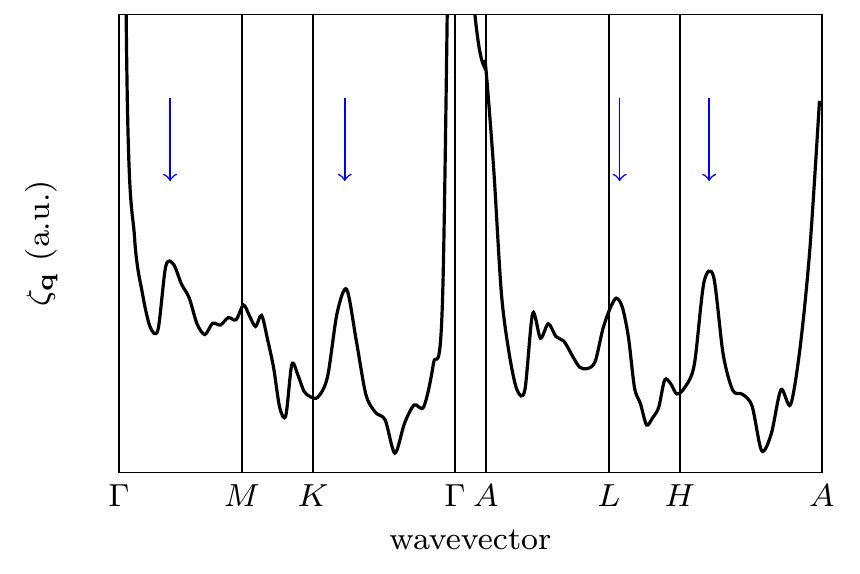
\includegraphics[width=0.5\textwidth]{figS3}
  \caption{(Color online) Calculated Fermi surface nesting function $\zeta_\mathbf{q}$ of 2$H$-NbS$_2$ along a high-symmetry path in the Brillouin zone, where the arrows point to local maxima. For a definition of the nesting function 
  see Ref.~\onlinecite{ponce_epw:_2016,heil_accurate_2014}. Peaks in this function can be used to identify nesting vectors, which connect parallel sheets of the Fermi surface (apart from ${\bf q}=0$, where the peak is an artifact of the definition). In this case, we do not find any clear indication of strong nesting inducing large EPI. The nesting function was calculated using a 200$\times$200$\times$100 Brillouin grid and a Gaussian smearing of 25~meV.}
  \end{figure}

\clearpage


  \begin{figure}[htbp]
  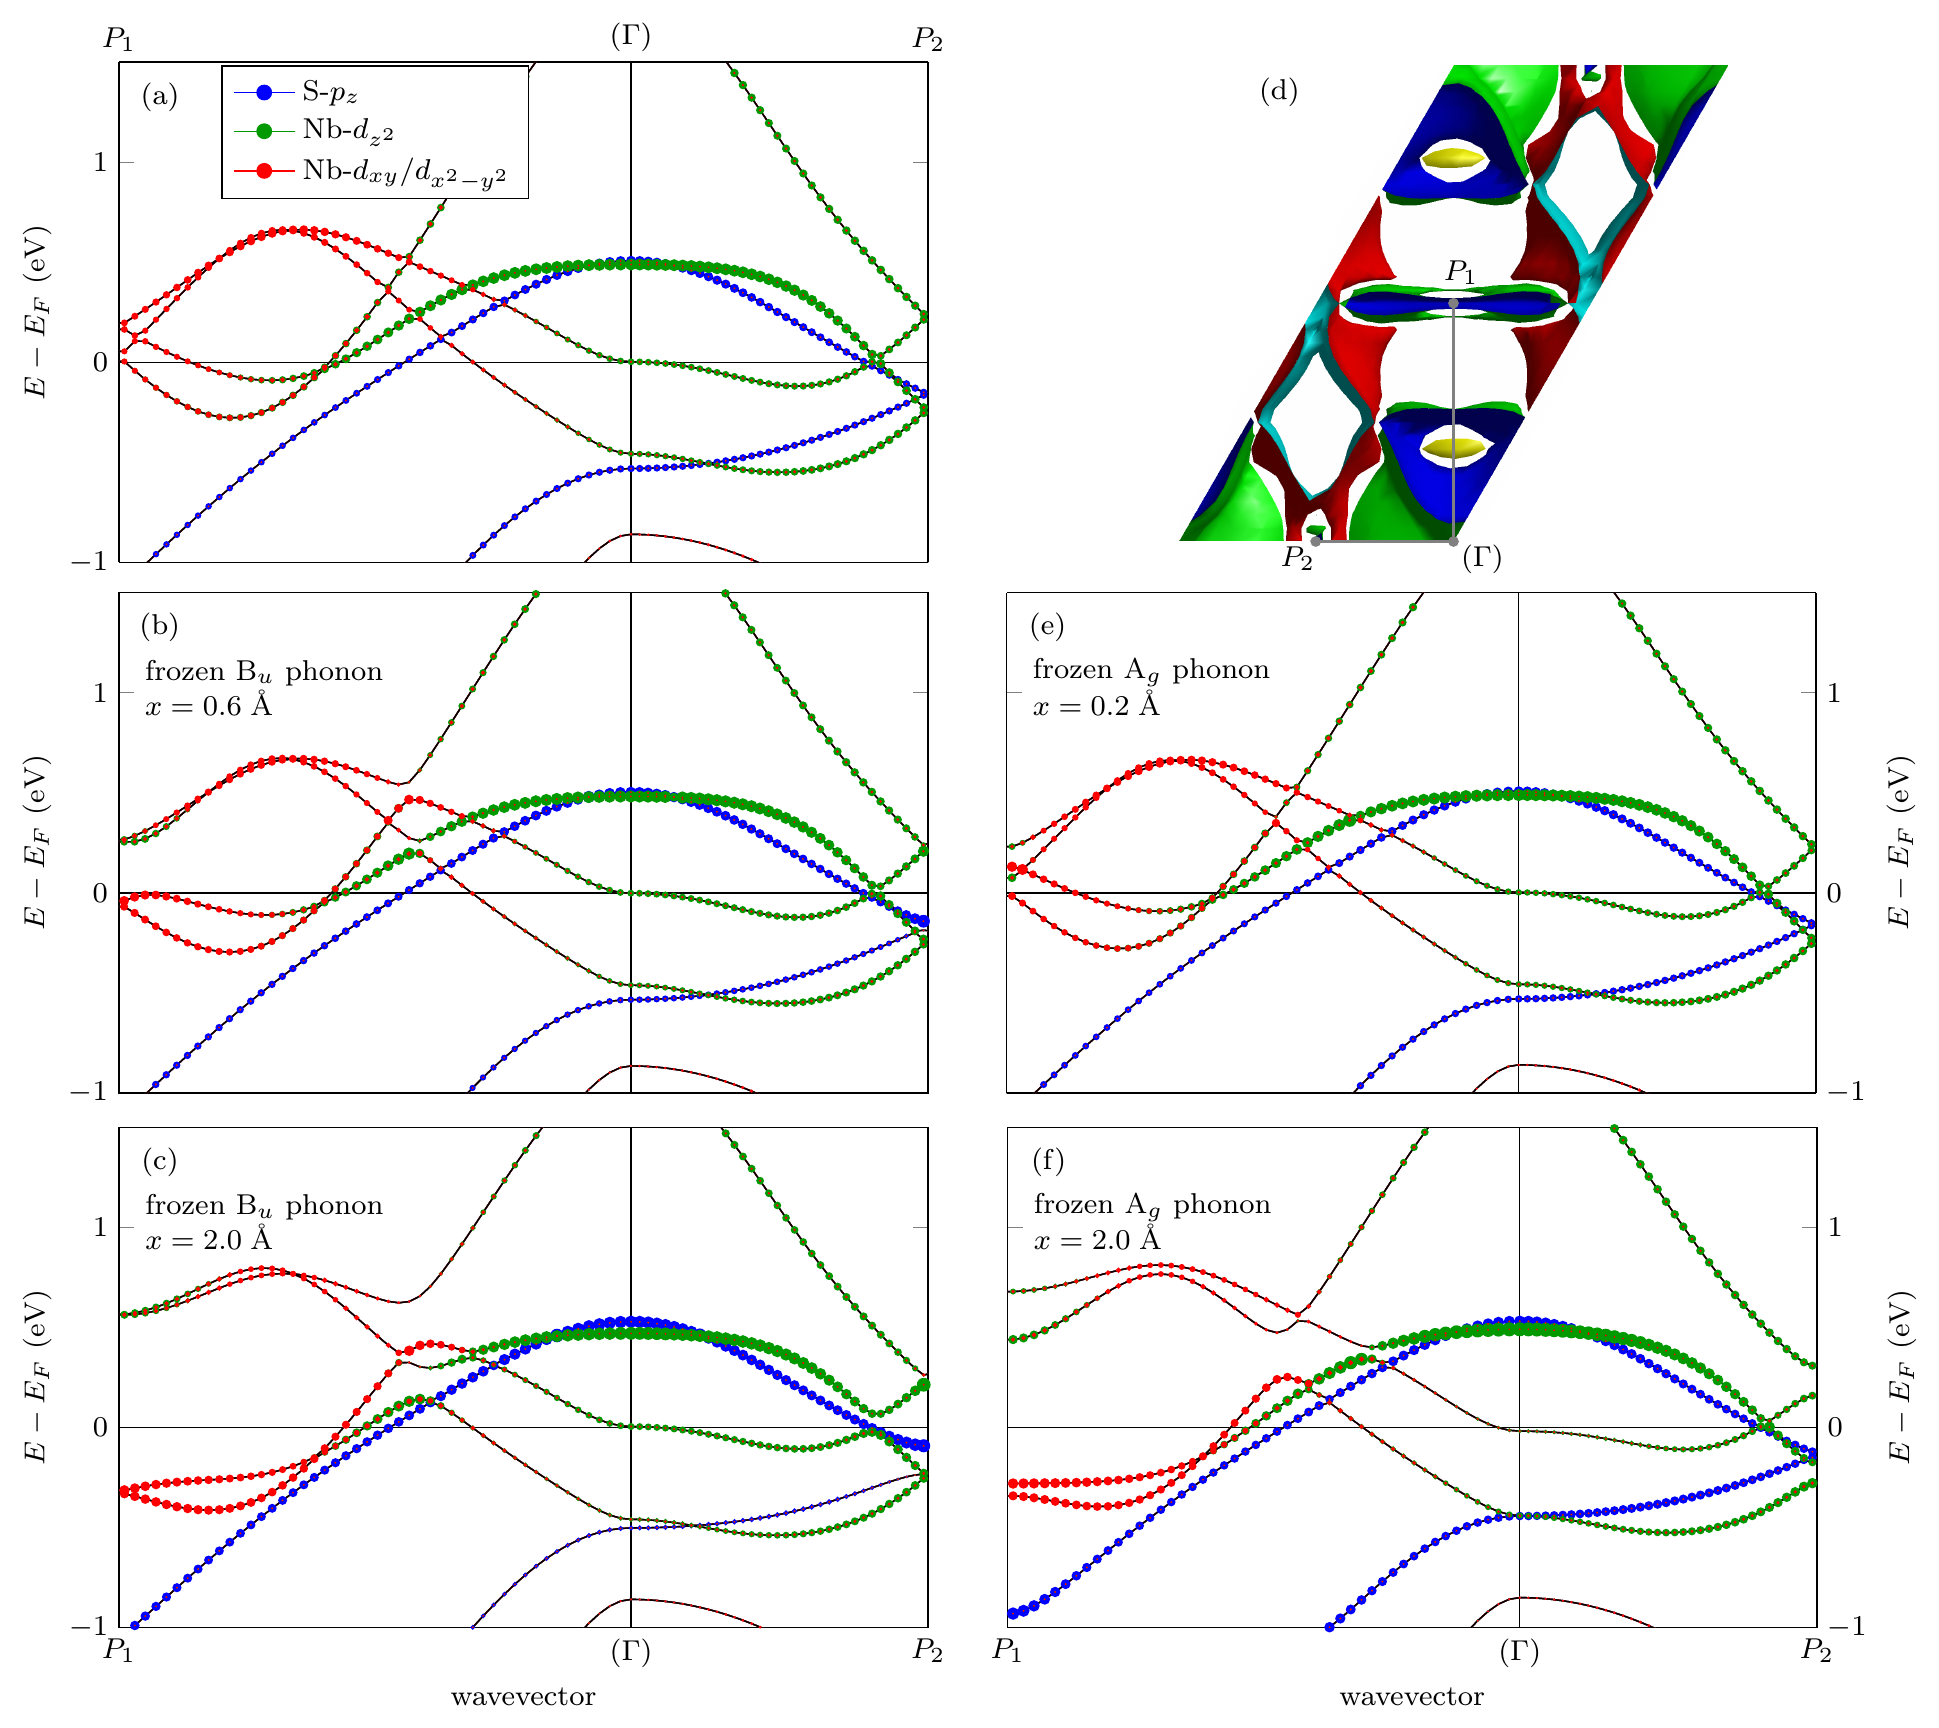
\includegraphics[width=1.0\textwidth]{figS4}
  \caption{(Color online)
  (a)-(c) Calculated band structure of 2$H$-NbS$_2$ in a $2\times1\times1$ supercell.
  In (a) we show the band structure in the ground state, in (b) the band structure calculated after displacing the atoms according to the B$_u$ phonon mode at $M$, so as to place the structure in one of the minima of the APES; and in (c) the band structure for a normal mode coordinate displacement of $x=2$~\r{A}, which corresponds to an absolute displacement of the Nb atoms of 0.1~\r{A} (see previous section on the anharmonic phonon calculations for a definition of the normal mode coordinate).  
  We see that the atomic displacement induces an avoided crossing in the band structure
  around the $P_1$ point with coordinates $(0.51,0.88,0.00)\;2\pi/a$. The splitting of electronic degeneracies and the removal of electronic states around the Fermi energy (compare with Fig.~S5) by a linear electron-phonon coupling is analogous to the dynamical Jahn-Teller effect in molecules~\cite{bersuker_jahn-teller_2006}, and is associated with a phonon softening and a latent lattice instability~\cite{katsnelson_singularities_1994,katsnelson_anomalies_1985}.
  (d) Calculated Fermi surfaces corresponding to the band structure in (a). The vibration of the $B_u$ phonon mode at $M$ modulates the shape of the Fermi surface, as it is seen in Fig.~3 of the main text.  
  (e)-(f) Similar to (b)-(c), but the atoms have been displaced according to the A$_g$ phonon mode.}
  \end{figure}



  \begin{figure}[htbp]
  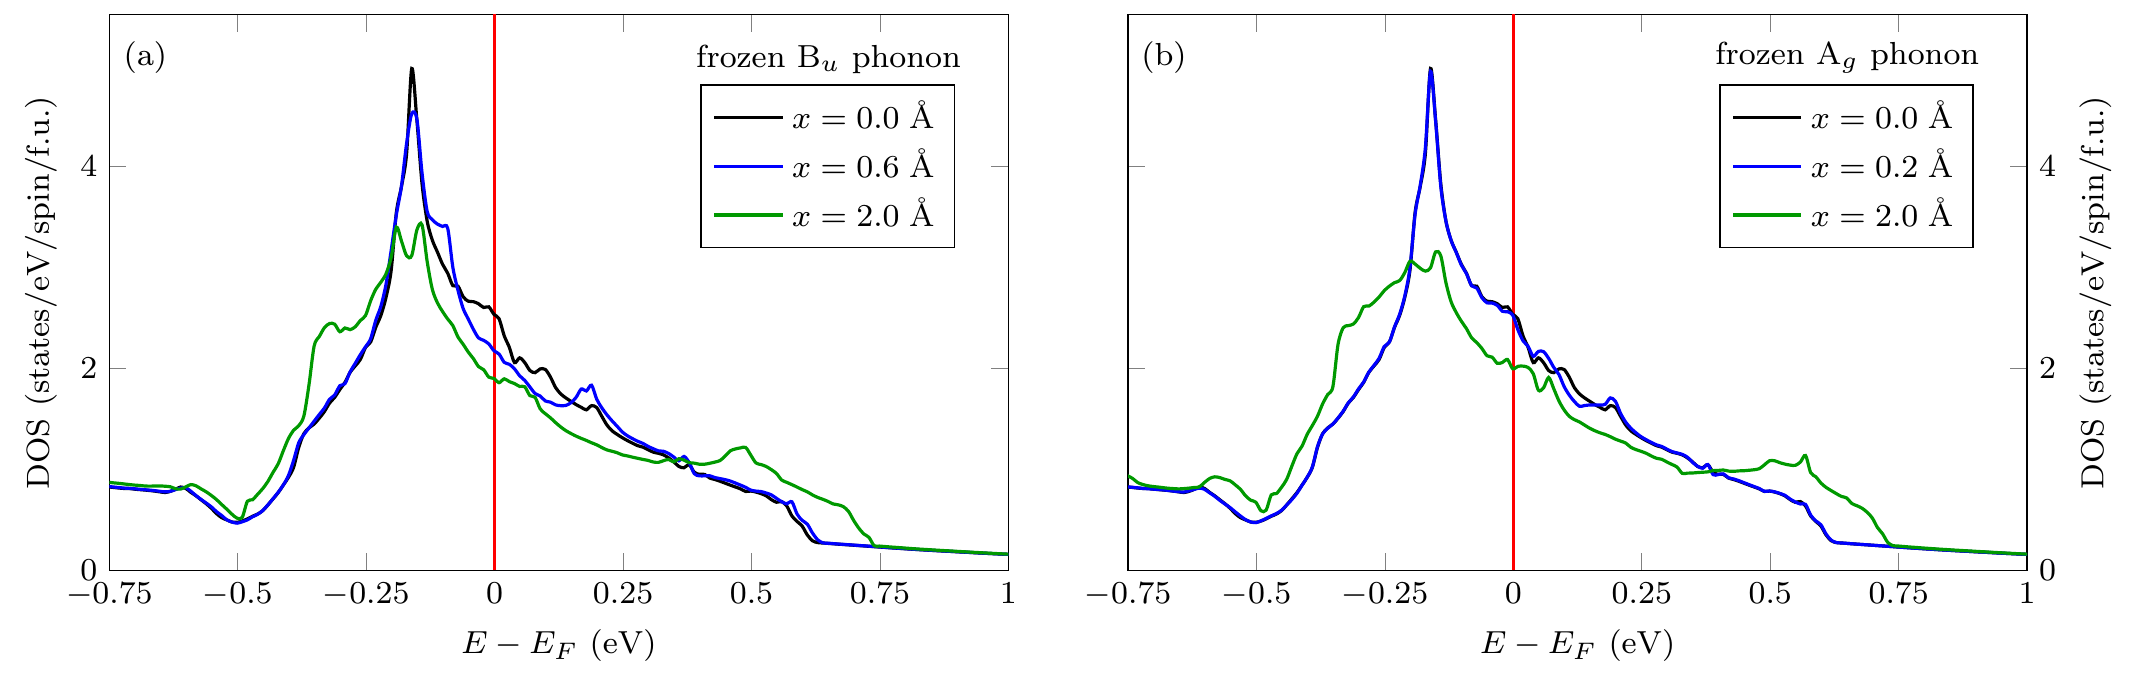
\includegraphics[width=1.0\textwidth]{figS5}
  \caption{(Color online)
  (a)-(b) Calculated DOS of 2$H$-NbS$_2$ in a $2\times1\times1$ supercell. In (a) we show the DOS in the ground state (black), and after displacing the atoms according to the B$_u$ phonon mode at $M$ for displacements of $x=0.6$\;\r{A} [blue; see also Eq.~(4)], which corresponds to placing the structure in the minimum of the anharmonic double-well potential, and $x=2.0$\;\r{A} (green), which corresponds to a displacement of the Nb atoms by $0.1$\;\r{A}. The DOS of the ground state structure exhibits a shoulder close to the Fermi energy, which is removed when the atoms are displaced along the B$_u$ mode. (b) Similar to (a), but the atoms have been displaced according to the A$_g$ phonon mode, with displacements of $x=0.2$\;\r{A} (blue) and $x=2.0$\;\r{A} (green). We observe a similar behavior as in (a), but not as pronounced. These figures show that the splitting of electronic degeneracies and the removal of electronic states from the Fermi level (compare with Fig.~S4) induce significant changes in the electronic structure of 2$H$-NbS$_2$ and play a role in the phonon softening in this compound~\cite{katsnelson_singularities_1994,katsnelson_anomalies_1985}.
  }
  \end{figure}

\clearpage

  
  \begin{figure}[htbp]
  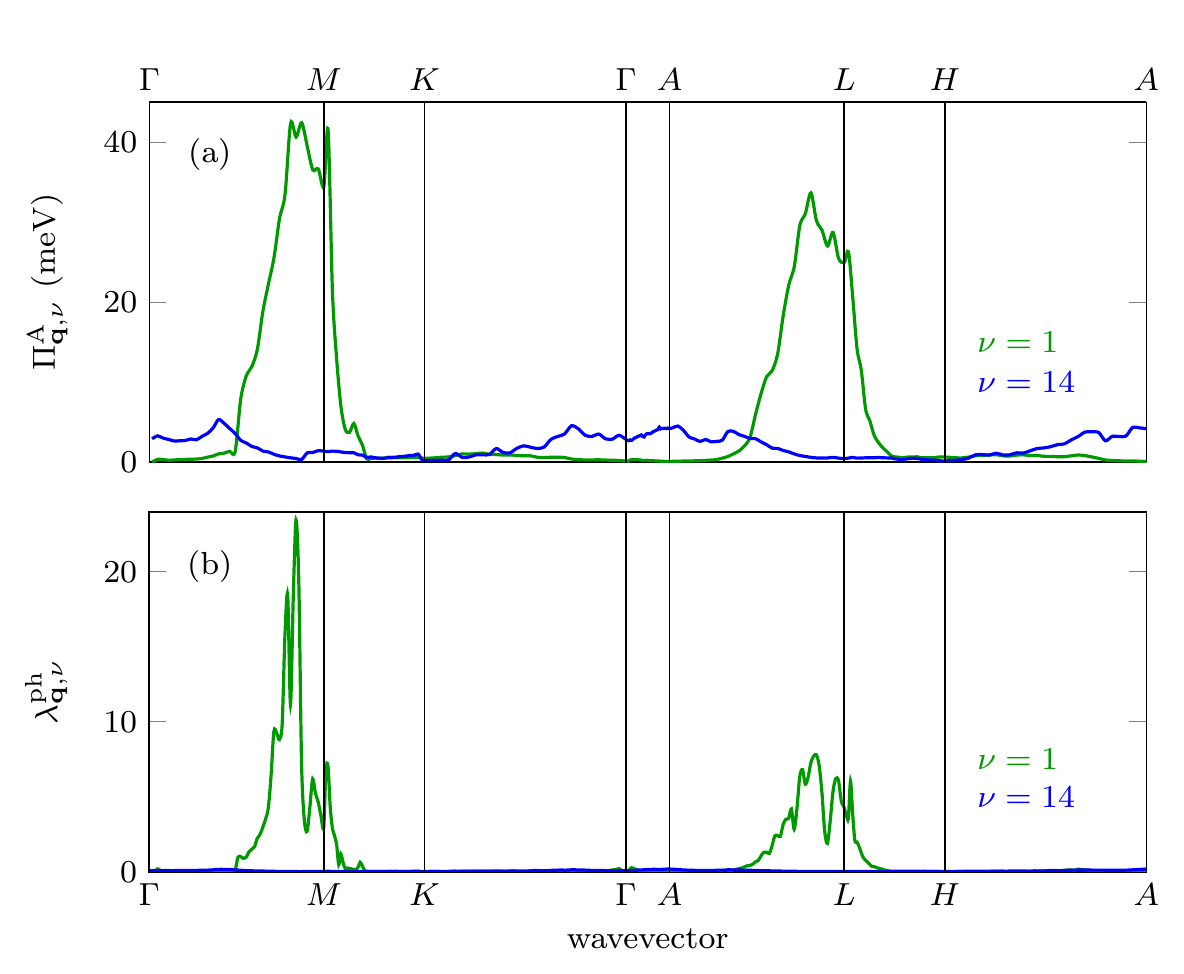
\includegraphics[width=0.7\textwidth]{figS6}
  \caption{(Color online) (a) The Fermi surface contribution to the adiabatic phonon self-energy~\cite{zhang_nonlocal_2005}\\ $\Pi_{\mathbf{q},\nu}^\text{A}=\sum \limits_{m,n} \int \frac{d\mathbf{k}}{\Omega_{\rm BZ}} |g_{mn,\nu}(\mathbf{k},\mathbf{q})|^2 \left[  \frac{f_{n,\mathbf{k}}-f_{m,\mathbf{k+q}}}{\epsilon_{m,\mathbf{k+q}} - \epsilon_{n,\mathbf{k}}} \right] \Theta(|\epsilon_{m,\mathbf{k+q}}-\epsilon_F|<\epsilon_c) \Theta(|\epsilon_{n,\mathbf{k}}-\epsilon_F|<\epsilon_c)$, \\with electron band indices $m,n$, phonon mode index $\nu$, reciprocal wavevectors $\mathbf{k} ,\mathbf{q}$, electron-phonon matrix elements $g_{mn,\nu}$, Fermi distribution function $f$, Brillouin zone volume $\Omega_{\rm BZ}$ and Fermi energy $\epsilon_F$. The step-function $\Theta$ with an energy cut-off $\epsilon_c=100$\;meV ensures that only electronic states close to $\epsilon_F$ are contributing to the self-energy, the qualitative results are insensitive to the choice of $\epsilon_c$. We observe that $\Pi_{\mathbf{q},\nu}^\text{A}$ for the first phonon mode (green) has large values in the vicinity of $2/3 \Gamma M$ ($2/3 AL$) and is close to zero everywhere else, while $\Pi_{\mathbf{q},\nu}^\text{A}$ for the 14$^{\rm th}$ phonon mode (blue) has a much lower and uniform response along the high-symmetry path. (b) EPI strength $\lambda_{\mathbf{q},\nu}^\text{ph}$ for the same two phonon modes as in (a). The fact that $\Pi_{\mathbf{q},\nu}^\text{A}$ is largest for those wavevectors $\mathbf{q}$ and phonon modes $\nu$ that also exhibit the largest EPI $\lambda_{\mathbf{q},\nu}^\text{ph}$ provides further evidence that the observed phonon softening is due to the large EPI associated with the anharmonic phonon modes in the vicinity of $2/3 \Gamma M$ ($2/3 AL$).}
  \end{figure}

\clearpage
  
  \begin{figure}[htbp]
  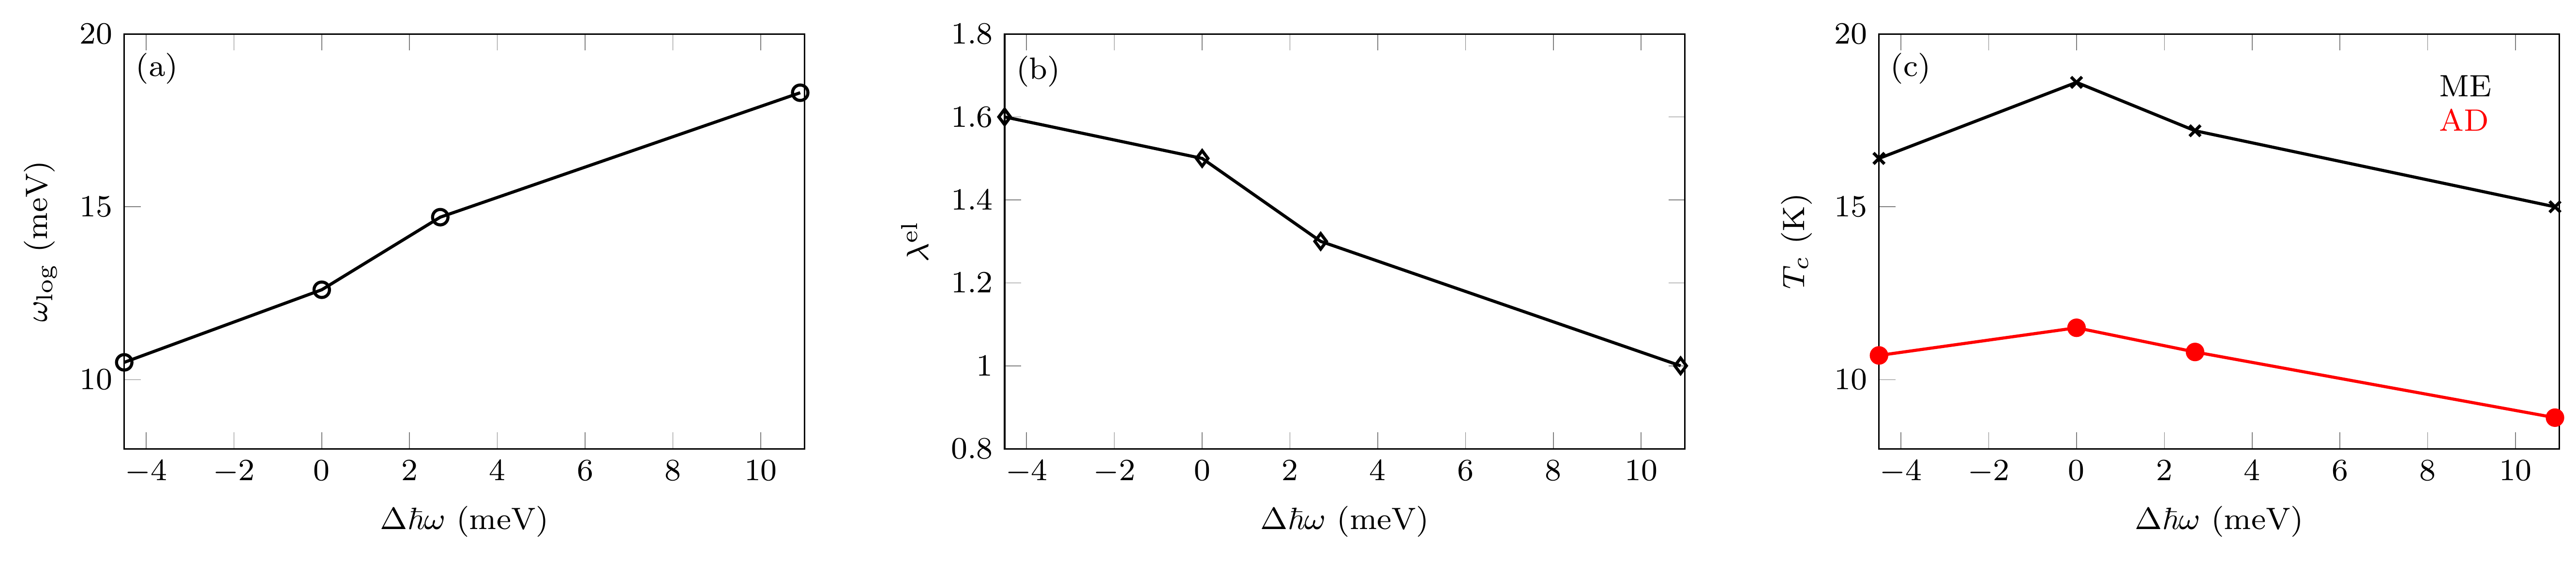
\includegraphics[width=1\textwidth]{figS7}
  \caption{(Color online) Sensitivity of the calculated superconducting properties of 2$H$-NbS$_2$ to the energy of the anharmonic modes. In panel (a) we show the logarithmic average phonon energy $\omega_\text{log}$ and in panel (b) the total EPI strength $\lambda^{\rm el}$ as a function of the energy shift $\Delta \hbar \omega$. In panel (c) we show the superconducting critical temperature calculated using the anisotropic Migdal-Eliashberg theory (`ME', black) and the Allen-Dynes formula (`AD', red) as a function of the energy shift $\Delta \hbar \omega$. In order to perform these calculations we rigidly shifted the energies of all the soft modes by the amount indicated on the horizontal axis. The critical temperature is found to be relatively insensitive to the phonon frequencies, owing to the compensating variations in $\omega_\text{log}$ and $\lambda^{\rm el}$.}
  \end{figure}


  \begin{figure}[htbp]
  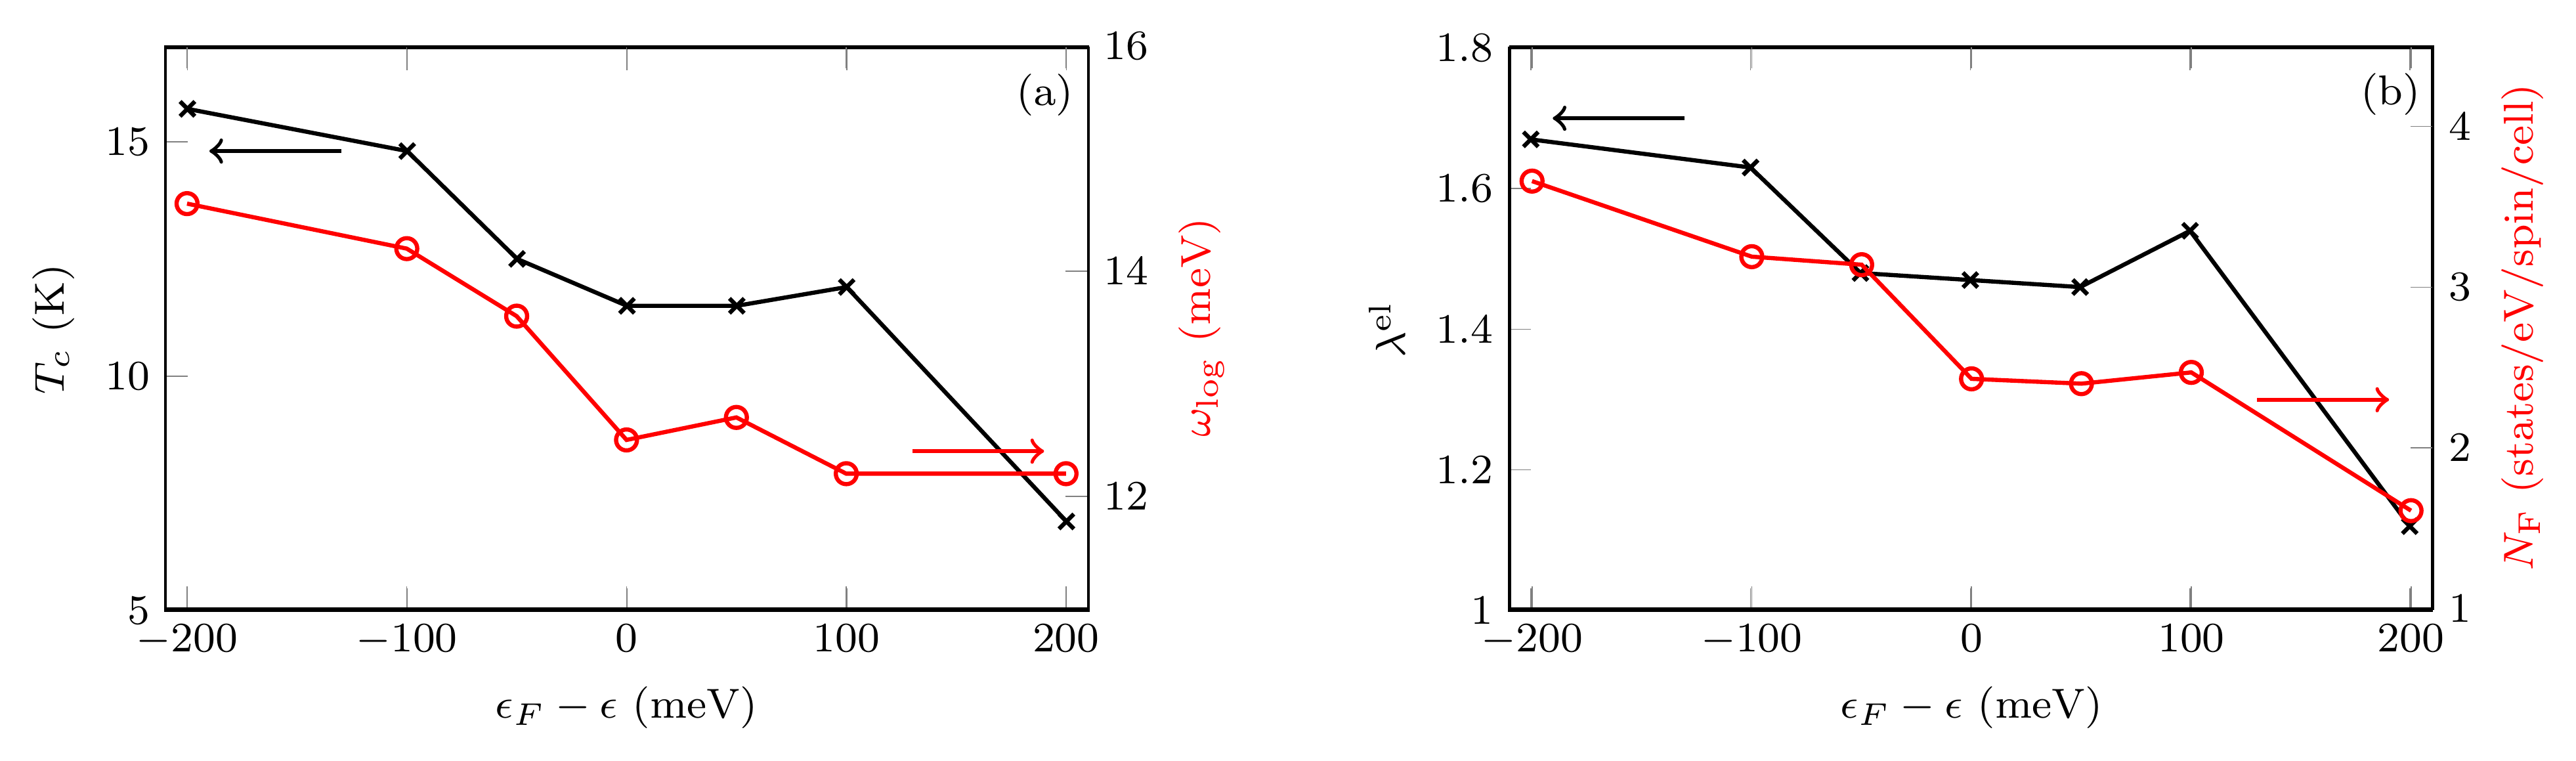
\includegraphics[width=0.8\textwidth]{figS8}
  \caption{(Color online)
  Sensitivity of the calculated superconducting properties of 2$H$-NbS$_2$ to the
  Fermi energy. (a) Variation of $T_{\rm c}$ calculated using the Allen-Dynes formula (black crosses) and of the logarithmic average phonon energy $\omega_\text{log}$ (red circles) 
  as a function of a rigid shift of the Fermi level. (b) Variation of the EPI strength $\lambda^{\rm el}$ (black crosses) and the DOS at the Fermi level (`$N_{\rm F}$', red circles) as a function of a rigid shift of the Fermi level. The large variation of the DOS with the Fermi energy has a significant impact on the calculated $T_{\rm c}$, mostly due to its effect on the EPI strength.}
  \end{figure}

\clearpage
  
  \begin{figure}[htbp]
  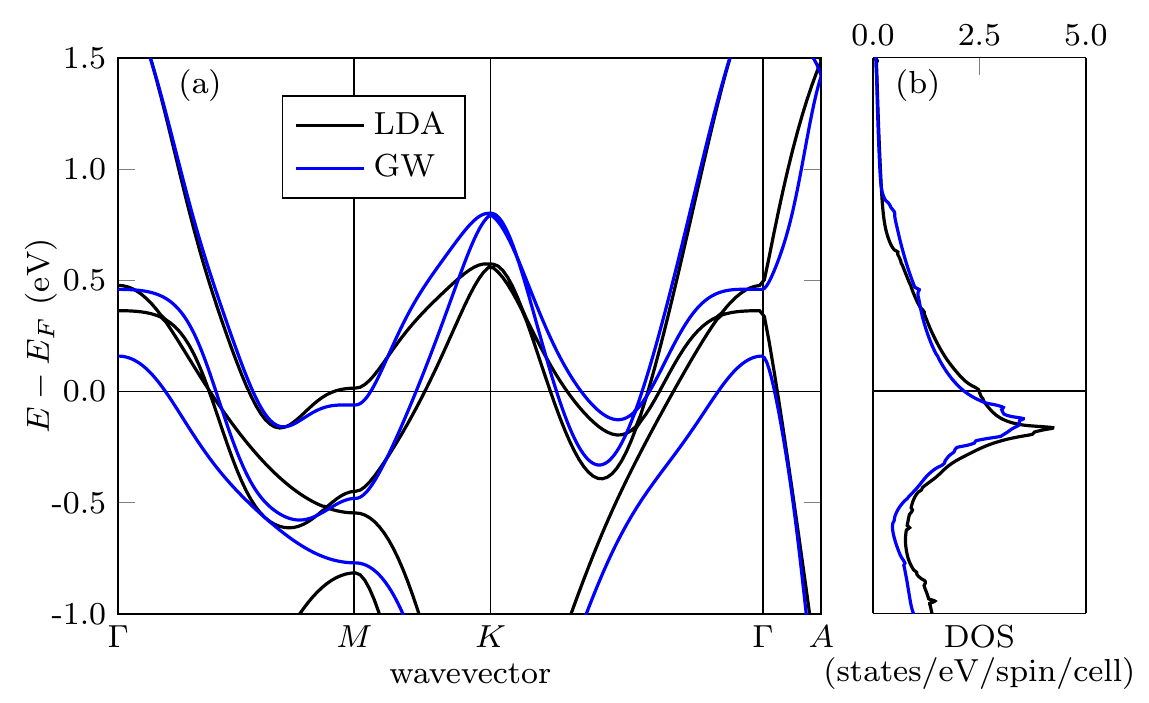
\includegraphics[width=0.6\textwidth]{figS9}
  \caption{(Color online)
  Comparison between calculations of the band structure (a) and density of states (b) of NbS$_2$ within the local density approximation to DFT (black) and within the $G_0W_0$ approximation as obtained using the SternheimerGW code (blue)~\cite{giustino_gw_2010,lambert_ab_2013}. The $G_0W_0$ calculations were performed using the Godby-Needs plasmon pole approximation~\cite{godby_metal-insulator_1989},
  using an imaginary pole energy of 4\;eV. The frequency integration was performed along the imaginary axis, and the self-energy on the real axis was obtained using analytic continuation based on Pad\'e approximants of order 11~\cite{giustino_gw_2010,lambert_ab_2013}. 
  For the screened Coulomb interaction we used a 12$\times$12$\times$4 Brillouin zone grid, 
  and we determined the quasiparticle corrections to the Kohn-Sham eigenvalues on a 6$\times$6$\times$2 Brillouin zone grid. These data were subsequently interpolated onto a fine 60$\times$60$\times$20 Brillouin zone grid by means of maximally localized Wannier functions~\cite{giustino_electron-phonon_2017,mostofi_wannier90:_2008}. We employed an energy cutoff of 10~Ry for the dielectric matrix, and an exchange self-energy cutoff 
  of 25~Ry. We note that the SternheimerGW method avoids the calculation of unoccupied electronic states, therefore no convergence over such states is required. The quasiparticle corrections decrease the DOS at the Fermi level by 18\%.}
  \end{figure}

  
  \begin{figure}[htbp]
  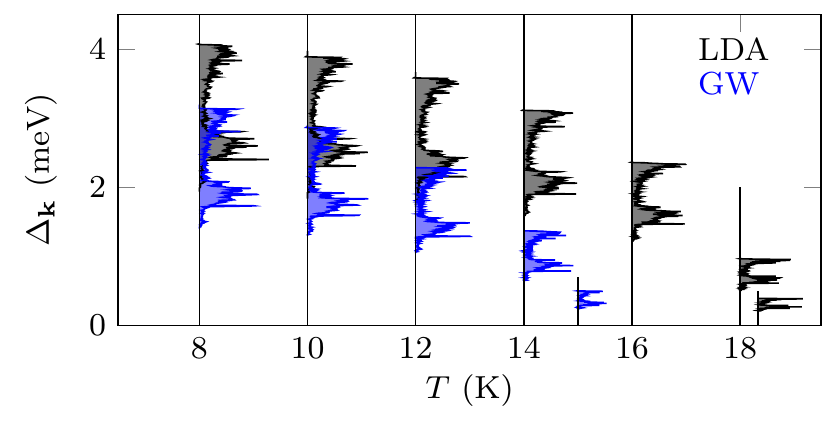
\includegraphics[width=0.6\textwidth]{figS10}
  \caption{(Color online)
  Calculated energy distribution of the superconducting gap $\Delta_\mathbf{k}$ as a function of temperature. The black curves (LDA) correspond to the result shown in Fig.~4(a) of the main text, the blue curves (GW) take into account the change in the DOS at the Fermi level due to GW quasiparticle corrections, as described in Fig.~S8. The quasiparticle corrections lower $T_{\rm c}$ by 18\%, from 18.6~K (LDA) to 15.3~K (GW). 
  Similarly the superconducting gap $\Delta_\mathbf{k}(T\rightarrow 0)$ decreases from $\sim 4.2$\;meV to $\sim 3.3$\;meV.}
  \end{figure}
  

\bibliographystyle{apsrev4-1}
% \bibliography{library}
%merlin.mbs apsrev4-1.bst 2010-07-25 4.21a (PWD, AO, DPC) hacked
%Control: key (0)
%Control: author (72) initials jnrlst
%Control: editor formatted (1) identically to author
%Control: production of article title (-1) disabled
%Control: page (0) single
%Control: year (1) truncated
%Control: production of eprint (0) enabled
\begin{thebibliography}{19}%
\makeatletter
\providecommand \@ifxundefined [1]{%
 \@ifx{#1\undefined}
}%
\providecommand \@ifnum [1]{%
 \ifnum #1\expandafter \@firstoftwo
 \else \expandafter \@secondoftwo
 \fi
}%
\providecommand \@ifx [1]{%
 \ifx #1\expandafter \@firstoftwo
 \else \expandafter \@secondoftwo
 \fi
}%
\providecommand \natexlab [1]{#1}%
\providecommand \enquote  [1]{``#1''}%
\providecommand \bibnamefont  [1]{#1}%
\providecommand \bibfnamefont [1]{#1}%
\providecommand \citenamefont [1]{#1}%
\providecommand \href@noop [0]{\@secondoftwo}%
\providecommand \href [0]{\begingroup \@sanitize@url \@href}%
\providecommand \@href[1]{\@@startlink{#1}\@@href}%
\providecommand \@@href[1]{\endgroup#1\@@endlink}%
\providecommand \@sanitize@url [0]{\catcode `\\12\catcode `\$12\catcode
  `\&12\catcode `\#12\catcode `\^12\catcode `\_12\catcode `\%12\relax}%
\providecommand \@@startlink[1]{}%
\providecommand \@@endlink[0]{}%
\providecommand \url  [0]{\begingroup\@sanitize@url \@url }%
\providecommand \@url [1]{\endgroup\@href {#1}{\urlprefix }}%
\providecommand \urlprefix  [0]{URL }%
\providecommand \Eprint [0]{\href }%
\providecommand \doibase [0]{http://dx.doi.org/}%
\providecommand \selectlanguage [0]{\@gobble}%
\providecommand \bibinfo  [0]{\@secondoftwo}%
\providecommand \bibfield  [0]{\@secondoftwo}%
\providecommand \translation [1]{[#1]}%
\providecommand \BibitemOpen [0]{}%
\providecommand \bibitemStop [0]{}%
\providecommand \bibitemNoStop [0]{.\EOS\space}%
\providecommand \EOS [0]{\spacefactor3000\relax}%
\providecommand \BibitemShut  [1]{\csname bibitem#1\endcsname}%
\let\auto@bib@innerbib\@empty
%</preamble>
\bibitem [{\citenamefont {Giustino}\ \emph {et~al.}(2007)\citenamefont
  {Giustino}, \citenamefont {Cohen},\ and\ \citenamefont
  {Louie}}]{giustino_electron-phonon_2007}%
  \BibitemOpen
  \bibfield  {author} {\bibinfo {author} {\bibfnamefont {F.}~\bibnamefont
  {Giustino}}, \bibinfo {author} {\bibfnamefont {M.~L.}\ \bibnamefont {Cohen}},
  \ and\ \bibinfo {author} {\bibfnamefont {S.~G.}\ \bibnamefont {Louie}},\
  }\href {\doibase 10.1103/PhysRevB.76.165108} {\bibfield  {journal} {\bibinfo
  {journal} {Phys. Rev. B}\ }\textbf {\bibinfo {volume} {76}},\ \bibinfo
  {pages} {165108} (\bibinfo {year} {2007})}\BibitemShut {NoStop}%
\bibitem [{\citenamefont {Lam}\ and\ \citenamefont
  {Cohen}(1982)}]{lam_ab_1982}%
  \BibitemOpen
  \bibfield  {author} {\bibinfo {author} {\bibfnamefont {P.~K.}\ \bibnamefont
  {Lam}}\ and\ \bibinfo {author} {\bibfnamefont {M.~L.}\ \bibnamefont
  {Cohen}},\ }\href {\doibase 10.1103/PhysRevB.25.6139} {\bibfield  {journal}
  {\bibinfo  {journal} {Phys. Rev. B}\ }\textbf {\bibinfo {volume} {25}},\
  \bibinfo {pages} {6139} (\bibinfo {year} {1982})}\BibitemShut {NoStop}%
\bibitem [{\citenamefont {Giustino}(2014)}]{giustino_materials_2014}%
  \BibitemOpen
  \bibfield  {author} {\bibinfo {author} {\bibfnamefont {F.}~\bibnamefont
  {Giustino}},\ }\href@noop {} {{\selectlanguage {English}\emph {\bibinfo
  {title} {Materials {Modelling} using {Density} {Functional} {Theory}:
  {Properties} and {Predictions}}}}}\ (\bibinfo  {publisher} {Oxford University
  Press},\ \bibinfo {address} {Oxford},\ \bibinfo {year} {2014})\BibitemShut
  {NoStop}%
\bibitem [{\citenamefont {Born}(1951)}]{born_fest._1951}%
  \BibitemOpen
  \bibfield  {author} {\bibinfo {author} {\bibfnamefont {M.}~\bibnamefont
  {Born}},\ }\href@noop {} {\emph {\bibinfo {title} {Fest. {Akad}. {D}. {Wiss}.
  {G\"{o}ttingen}: {I}. {Math}.-{Phys}. {Klasse}}}},\ \bibinfo {edition} {1951st}\
  ed.\ (\bibinfo  {publisher} {Springer},\ \bibinfo {year} {1951})\BibitemShut
  {NoStop}%
\bibitem [{\citenamefont {Hooton}(1955)}]{hooton_li._1955}%
  \BibitemOpen
  \bibfield  {author} {\bibinfo {author} {\bibfnamefont {D.~J.}\ \bibnamefont
  {Hooton}},\ }\href {\doibase 10.1080/14786440408520575} {\bibfield  {journal}
  {\bibinfo  {journal} {Phil. Mag.}\ }\textbf {\bibinfo {volume} {46}},\
  \bibinfo {pages} {422} (\bibinfo {year} {1955})}\BibitemShut {NoStop}%
\bibitem [{\citenamefont {Koehler}(1966)}]{koehler_theory_1966}%
  \BibitemOpen
  \bibfield  {author} {\bibinfo {author} {\bibfnamefont {T.~R.}\ \bibnamefont
  {Koehler}},\ }\href {\doibase 10.1103/PhysRevLett.17.89} {\bibfield
  {journal} {\bibinfo  {journal} {Phys. Rev. Lett.}\ }\textbf {\bibinfo
  {volume} {17}},\ \bibinfo {pages} {89} (\bibinfo {year} {1966})}\BibitemShut
  {NoStop}%
\bibitem [{\citenamefont {Souvatzis}\ \emph {et~al.}(2008)\citenamefont
  {Souvatzis}, \citenamefont {Eriksson}, \citenamefont {Katsnelson},\ and\
  \citenamefont {Rudin}}]{souvatzis_entropy_2008}%
  \BibitemOpen
  \bibfield  {author} {\bibinfo {author} {\bibfnamefont {P.}~\bibnamefont
  {Souvatzis}}, \bibinfo {author} {\bibfnamefont {O.}~\bibnamefont {Eriksson}},
  \bibinfo {author} {\bibfnamefont {M.~I.}\ \bibnamefont {Katsnelson}}, \ and\
  \bibinfo {author} {\bibfnamefont {S.~P.}\ \bibnamefont {Rudin}},\ }\href
  {\doibase 10.1103/PhysRevLett.100.095901} {\bibfield  {journal} {\bibinfo
  {journal} {Phys. Rev. Lett.}\ }\textbf {\bibinfo {volume} {100}},\ \bibinfo
  {pages} {095901} (\bibinfo {year} {2008})}\BibitemShut {NoStop}%
\bibitem [{\citenamefont {Errea}\ \emph {et~al.}(2013)\citenamefont {Errea},
  \citenamefont {Calandra},\ and\ \citenamefont
  {Mauri}}]{errea_first-principles_2013}%
  \BibitemOpen
  \bibfield  {author} {\bibinfo {author} {\bibfnamefont {I.}~\bibnamefont
  {Errea}}, \bibinfo {author} {\bibfnamefont {M.}~\bibnamefont {Calandra}}, \
  and\ \bibinfo {author} {\bibfnamefont {F.}~\bibnamefont {Mauri}},\ }\href
  {\doibase 10.1103/PhysRevLett.111.177002} {\bibfield  {journal} {\bibinfo
  {journal} {Phys. Rev. Lett.}\ }\textbf {\bibinfo {volume} {111}},\ \bibinfo
  {pages} {177002} (\bibinfo {year} {2013})}\BibitemShut {NoStop}%
\bibitem [{\citenamefont {Ponc\'{e}}\ \emph {et~al.}(2016)\citenamefont
  {Ponc\'{e}}, \citenamefont {Margine}, \citenamefont {Verdi},\ and\
  \citenamefont {Giustino}}]{ponce_epw:_2016}%
  \BibitemOpen
  \bibfield  {author} {\bibinfo {author} {\bibfnamefont {S.}~\bibnamefont
  {Ponc\'{e}}}, \bibinfo {author} {\bibfnamefont {E.~R.}\ \bibnamefont
  {Margine}}, \bibinfo {author} {\bibfnamefont {C.}~\bibnamefont {Verdi}}, \
  and\ \bibinfo {author} {\bibfnamefont {F.}~\bibnamefont {Giustino}},\ }\href
  {\doibase 10.1016/j.cpc.2016.07.028} {\bibfield  {journal} {\bibinfo
  {journal} {Comput. Phys. Commun.}\ }\textbf {\bibinfo {volume} {209}},\
  \bibinfo {pages} {116} (\bibinfo {year} {2016})}\BibitemShut {NoStop}%
\bibitem [{\citenamefont {Heil}\ \emph {et~al.}(2014)\citenamefont {Heil},
  \citenamefont {Sormann}, \citenamefont {Boeri}, \citenamefont {Aichhorn},\
  and\ \citenamefont {von~der Linden}}]{heil_accurate_2014}%
  \BibitemOpen
  \bibfield  {author} {\bibinfo {author} {\bibfnamefont {C.}~\bibnamefont
  {Heil}}, \bibinfo {author} {\bibfnamefont {H.}~\bibnamefont {Sormann}},
  \bibinfo {author} {\bibfnamefont {L.}~\bibnamefont {Boeri}}, \bibinfo
  {author} {\bibfnamefont {M.}~\bibnamefont {Aichhorn}}, \ and\ \bibinfo
  {author} {\bibfnamefont {W.}~\bibnamefont {von~der Linden}},\ }\href
  {\doibase 10.1103/PhysRevB.90.115143} {\bibfield  {journal} {\bibinfo
  {journal} {Phys. Rev. B}\ }\textbf {\bibinfo {volume} {90}},\ \bibinfo
  {pages} {115143} (\bibinfo {year} {2014})}\BibitemShut {NoStop}%
\bibitem [{\citenamefont {Bersuker}(2006)}]{bersuker_jahn-teller_2006}%
  \BibitemOpen
  \bibfield  {author} {\bibinfo {author} {\bibfnamefont {I.~C.}\ \bibnamefont
  {Bersuker}},\ }\href@noop {} {{\selectlanguage {English}\emph {\bibinfo
  {title} {The {Jahn}-{Teller} {Effect}}}}},\ \bibinfo {edition} {reissue
  edition}\ ed.\ (\bibinfo  {publisher} {Cambridge University Press},\ \bibinfo
  {address} {Cambridge},\ \bibinfo {year} {2006})\BibitemShut {NoStop}%
\bibitem [{\citenamefont {Katsnelson}\ \emph {et~al.}(1994)\citenamefont
  {Katsnelson}, \citenamefont {Naumov},\ and\ \citenamefont
  {Trefilov}}]{katsnelson_singularities_1994}%
  \BibitemOpen
  \bibfield  {author} {\bibinfo {author} {\bibfnamefont {M.~I.}\ \bibnamefont
  {Katsnelson}}, \bibinfo {author} {\bibfnamefont {I.~I.}\ \bibnamefont
  {Naumov}}, \ and\ \bibinfo {author} {\bibfnamefont {A.~V.}\ \bibnamefont
  {Trefilov}},\ }\href {\doibase 10.1080/01411599408201172} {\bibfield
  {journal} {\bibinfo  {journal} {Phase Transit.}\ }\textbf {\bibinfo
  {volume} {49}},\ \bibinfo {pages} {143} (\bibinfo {year} {1994})}\BibitemShut
  {NoStop}%
\bibitem [{\citenamefont {Katsnelson}(1985)}]{katsnelson_anomalies_1985}%
  \BibitemOpen
  \bibfield  {author} {\bibinfo {author} {\bibfnamefont {M.~I.}~\bibnamefont
  {Katsnelson}}, \ and\ \bibinfo {author} {\bibfnamefont {A.~V.}\ \bibnamefont {Trefilov}},\ } {\bibfield  {journal}
  {\bibinfo  {journal} {JETP Lett.}\ }\textbf {\bibinfo {volume} {42}},\
  \bibinfo {pages} {485} (\bibinfo {year} {1985})}\BibitemShut {NoStop}%
\bibitem [{\citenamefont {Zhang}\ \emph {et~al.}(2005)\citenamefont {Zhang},
  \citenamefont {Louie},\ and\ \citenamefont {Cohen}}]{zhang_nonlocal_2005}%
  \BibitemOpen
  \bibfield  {author} {\bibinfo {author} {\bibfnamefont {P.}~\bibnamefont
  {Zhang}}, \bibinfo {author} {\bibfnamefont {S.~G.}\ \bibnamefont {Louie}}, \
  and\ \bibinfo {author} {\bibfnamefont {M.~L.}\ \bibnamefont {Cohen}},\ }\href
  {\doibase 10.1103/PhysRevLett.94.225502} {\bibfield  {journal} {\bibinfo
  {journal} {Phys. Rev. Lett.}\ }\textbf {\bibinfo {volume} {94}},\ \bibinfo
  {pages} {225502} (\bibinfo {year} {2005})}\BibitemShut {NoStop}%
\bibitem [{\citenamefont {Giustino}\ \emph {et~al.}(2010)\citenamefont
  {Giustino}, \citenamefont {Cohen},\ and\ \citenamefont
  {Louie}}]{giustino_gw_2010}%
  \BibitemOpen
  \bibfield  {author} {\bibinfo {author} {\bibfnamefont {F.}~\bibnamefont
  {Giustino}}, \bibinfo {author} {\bibfnamefont {M.~L.}\ \bibnamefont {Cohen}},
  \ and\ \bibinfo {author} {\bibfnamefont {S.~G.}\ \bibnamefont {Louie}},\
  }\href {\doibase 10.1103/PhysRevB.81.115105} {\bibfield  {journal} {\bibinfo
  {journal} {Phys. Rev. B}\ }\textbf {\bibinfo {volume} {81}},\ \bibinfo
  {pages} {115105} (\bibinfo {year} {2010})}\BibitemShut {NoStop}%
\bibitem [{\citenamefont {Lambert}\ and\ \citenamefont
  {Giustino}(2013)}]{lambert_ab_2013}%
  \BibitemOpen
  \bibfield  {author} {\bibinfo {author} {\bibfnamefont {H.}~\bibnamefont
  {Lambert}}\ and\ \bibinfo {author} {\bibfnamefont {F.}~\bibnamefont
  {Giustino}},\ }\href {\doibase 10.1103/PhysRevB.88.075117} {\bibfield
  {journal} {\bibinfo  {journal} {Phys. Rev. B}\ }\textbf {\bibinfo {volume}
  {88}},\ \bibinfo {pages} {075117} (\bibinfo {year} {2013})}\BibitemShut
  {NoStop}%
\bibitem [{\citenamefont {Godby}\ and\ \citenamefont
  {Needs}(1989)}]{godby_metal-insulator_1989}%
  \BibitemOpen
  \bibfield  {author} {\bibinfo {author} {\bibfnamefont {R.~W.}\ \bibnamefont
  {Godby}}\ and\ \bibinfo {author} {\bibfnamefont {R.~J.}\ \bibnamefont
  {Needs}},\ }\href {\doibase 10.1103/PhysRevLett.62.1169} {\bibfield
  {journal} {\bibinfo  {journal} {Phys. Rev. Lett.}\ }\textbf {\bibinfo
  {volume} {62}},\ \bibinfo {pages} {1169} (\bibinfo {year}
  {1989})}\BibitemShut {NoStop}%
\bibitem [{\citenamefont {Giustino}(2017)}]{giustino_electron-phonon_2017}%
  \BibitemOpen
  \bibfield  {author} {\bibinfo {author} {\bibfnamefont {F.}~\bibnamefont
  {Giustino}},\ }\href {\doibase 10.1103/RevModPhys.89.015003} {\bibfield
  {journal} {\bibinfo  {journal} {Rev. Mod. Phys.}\ }\textbf {\bibinfo {volume}
  {89}},\ \bibinfo {pages} {015003} (\bibinfo {year} {2017})}\BibitemShut
  {NoStop}%
\bibitem [{\citenamefont {Mostofi}\ \emph {et~al.}(2008)\citenamefont
  {Mostofi}, \citenamefont {Yates}, \citenamefont {Lee}, \citenamefont {Souza},
  \citenamefont {Vanderbilt},\ and\ \citenamefont
  {Marzari}}]{mostofi_wannier90:_2008}%
  \BibitemOpen
  \bibfield  {author} {\bibinfo {author} {\bibfnamefont {A.~A.}\ \bibnamefont
  {Mostofi}}, \bibinfo {author} {\bibfnamefont {J.~R.}\ \bibnamefont {Yates}},
  \bibinfo {author} {\bibfnamefont {Y.-S.}\ \bibnamefont {Lee}}, \bibinfo
  {author} {\bibfnamefont {I.}~\bibnamefont {Souza}}, \bibinfo {author}
  {\bibfnamefont {D.}~\bibnamefont {Vanderbilt}}, \ and\ \bibinfo {author}
  {\bibfnamefont {N.}~\bibnamefont {Marzari}},\ }\href {\doibase
  10.1016/j.cpc.2007.11.016} {\bibfield  {journal} {\bibinfo  {journal}
  {Comput. Phys. Commun.}\ }\textbf {\bibinfo {volume} {178}},\
  \bibinfo {pages} {685} (\bibinfo {year} {2008})}\BibitemShut {NoStop}%
\end{thebibliography}%
\end{document}



